%\chapter*{Erkl�rung}
%\thispagestyle{empty}
%\hypertarget{hypsec:erklaerung_der_selbstst}{}%
%
%Ich versichere hiermit, dass ich die vorliegende Arbeit selbstst�ndig
%und ohne Benutzung anderer als der angegebenen Hilfsmittel angefertigt
%habe. Alle Stellen, die w�rtlich oder sinngem�� aus
%ver�ffentlichten und nicht ver�ffentlichten Schriften entnommen
%sind, wurden als solche kenntlich gemacht.\\[3cm]
%
%\begin{tabularx}{\textwidth}{lXl}
%  \rule{5cm}{0.4pt} & & \rule{5cm}{0.4pt}\\
%  Ort, Datum & & Unterschrift
%\end{tabularx}
%\includepdf[angle=90,landscape]{Testbild.png}
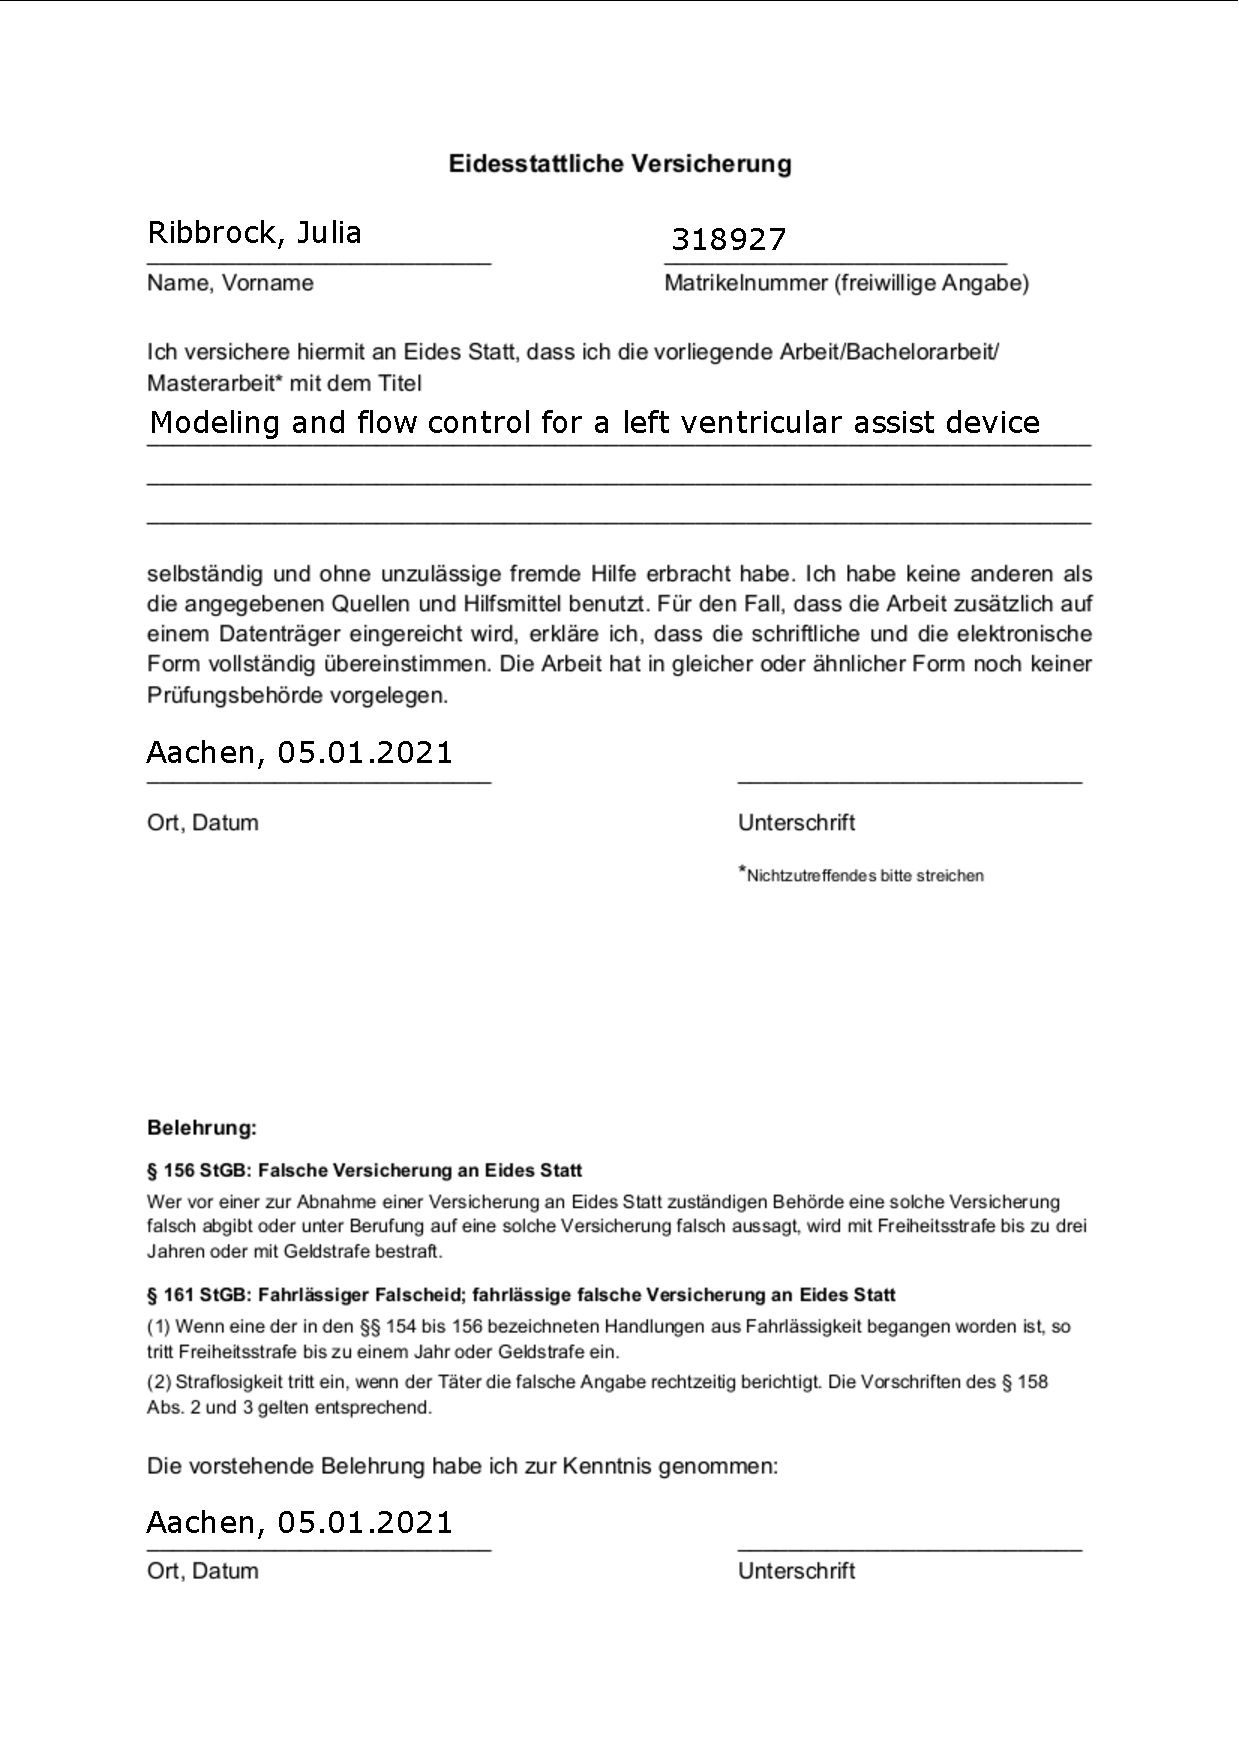
\includepdf{images/Formular_Eidesstattliche_Versicherung_neu_2}

%\begin{figure}[!ht]
%  \centering
%   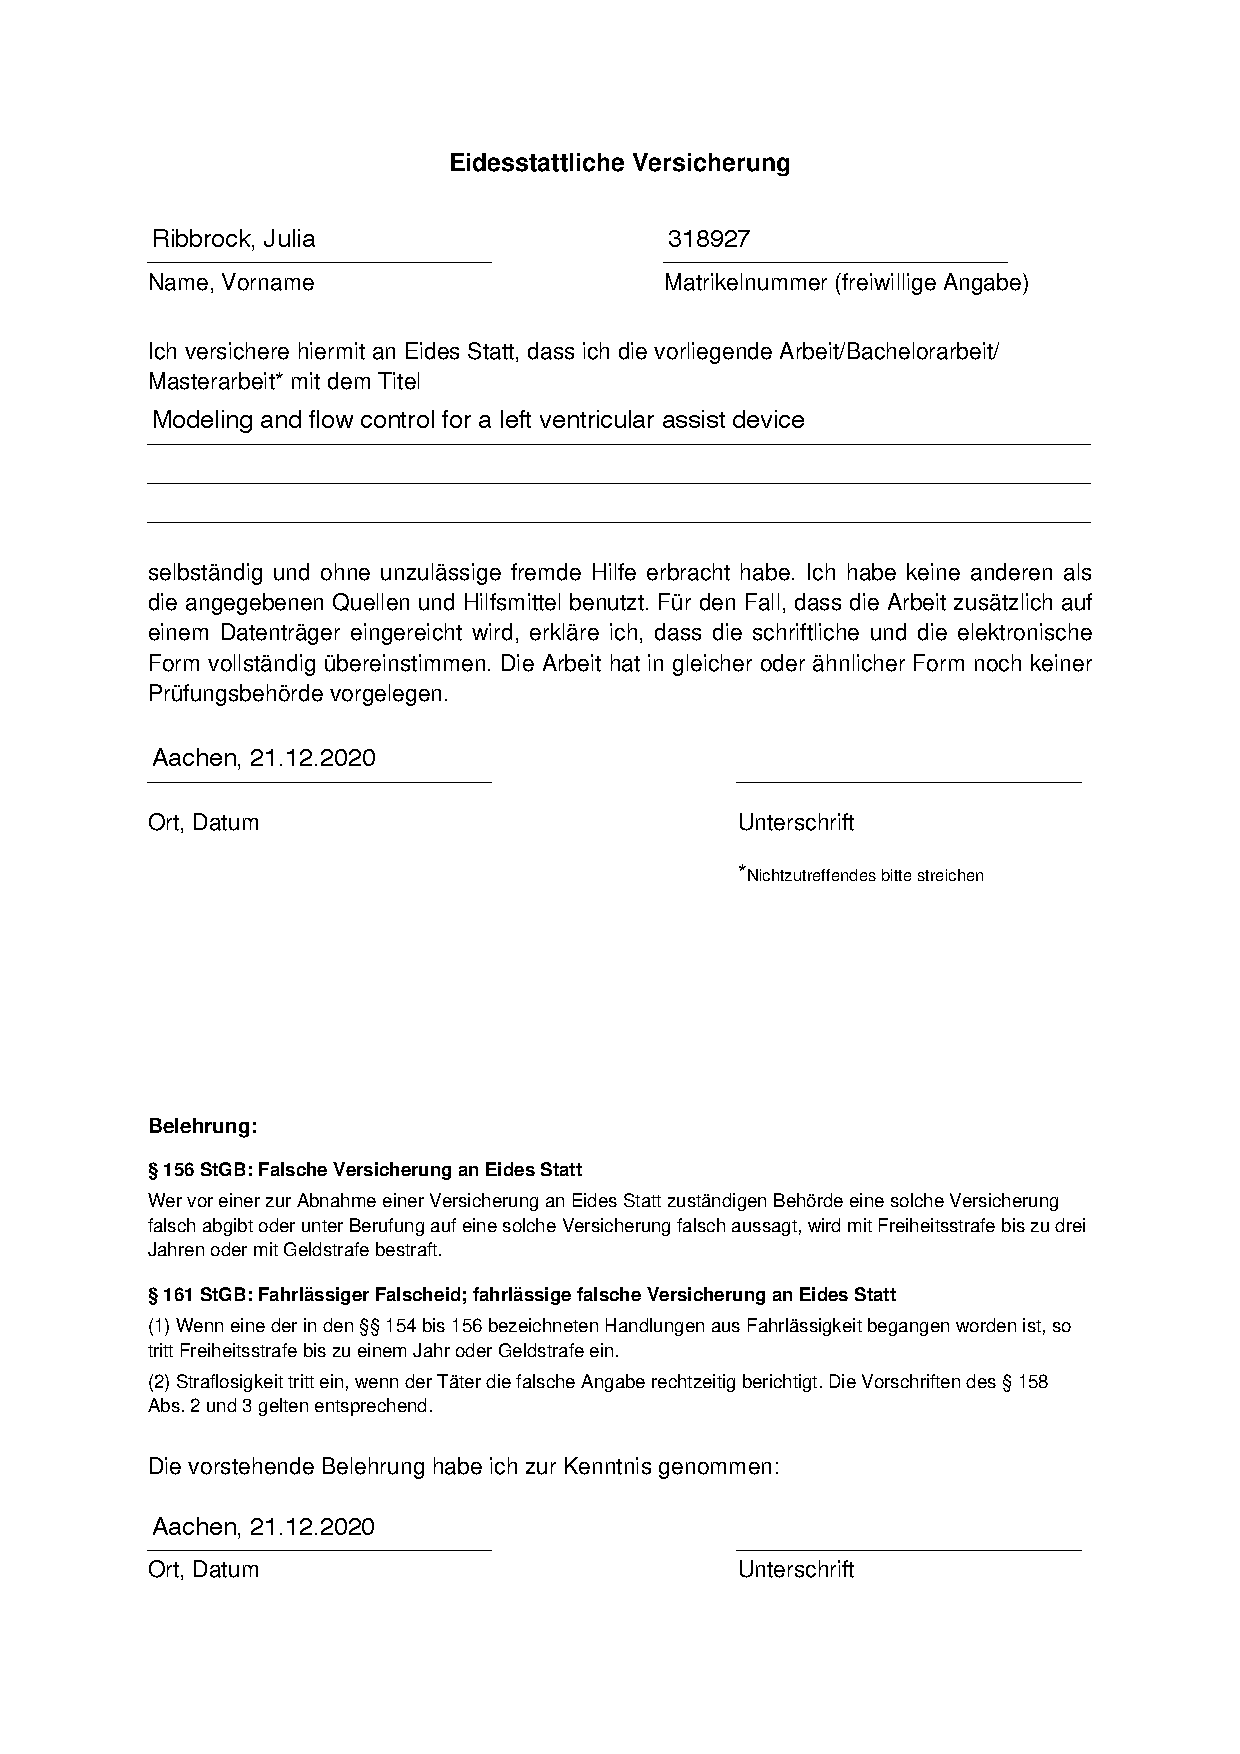
\includegraphics[scale=1]{images/Formular_Eidesstattliche_Versicherung_neu}
%   % Die folgende Anweisungen bindet die Grafik nocheinmal zus�tzlich
%   % als Dateianhang ein. Das hat den Vorteil, dass sie einfach aus dem pdf zur
%   % wieterverwendung extrahierbar ist und der Autor (author) mit angegeben
%   % werden kann. Leider ist die Grafik dadurch auch gleich zweimal im pdf
%   % enthalten und verbraucht dadurch doppelt Platz.
%   % \textattachfile[mimetype=application/pdf,print=false,author=\docauthor,description=\figurename~\ref{fig:beispiel1}]{beispiel1.pdf}{}
%  %% Reihenfolge der Befehle wichtig: zuerst die \caption, danach das \label
%  \label{fig:EidesstattlicheVersicherung}
%\end{figure}
